\documentclass[paper=a4,fontsize=12pt]{scrartcl}
					
\usepackage[english]{babel}
\usepackage{graphicx}     
\usepackage[svgnames]{xcolor}    
\usepackage{geometry}
	\textheight=700px          

\frenchspacing             
\pagestyle{empty}         


\newlength{\spacebox}
\settowidth{\spacebox}{8888888888}		
\newcommand{\sepspace}{\vspace*{1em}}

\newcommand{\Title}[1]{
		\Huge \usefont{OT1}{phv}{b}{n} \hfill #1
		\par \normalsize \normalfont}
		
\newcommand{\Subtitle}[1]{ 
		\large \usefont{OT1}{phv}{m}{n}\hfill \textit{#1}
		\par \normalsize \normalfont}

\newcommand{\NewPart}[1]{\section*{\uppercase{#1}}}

\newcommand{\AccountEntry}[2]{
		\noindent\hangindent=2em\hangafter=0 
		\parbox{\spacebox}{ 
		\textit{#1}}
		\hspace{1.5em} #2 \par}
		
\newcommand{\EducationEntry}[4]{
		\noindent \textbf{#1} \hfill  
		\noindent \textit{#2}
		\colorbox{Black}{%
			\parbox{6em}{%
			\hfill\color{White}#3}} \par
		\normalsize \par}

\begin{document}
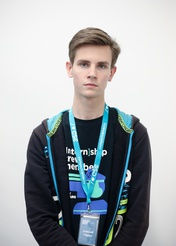
\includegraphics[width=0.3\textwidth]{img.jpg}

\Title{Aleksey Pauls}
\Subtitle{Student of 2018 admission}

\NewPart{About}{}

I study in CSC on "Data Analysis" because I`m interested in artificial intelligence 
and everything related to it: machine learning, deep learning, statistics, NLP, etc.

\NewPart{Accounts}{}

\AccountEntry{Email}{a.pauls@g.nsu.ru}
\AccountEntry{Github}{AlekseyPauls}
\AccountEntry{Stepik}{47096585}

\NewPart{Curses}{}

\EducationEntry{Algorithms and data structures, part 1}{Autumn 2018}{Good}

\EducationEntry{Discrete analysis and probability theory}{Autumn 2018}{Good}

\EducationEntry{Python Programming}{Autumn 2018}{Good}

\EducationEntry{Machine Learning, Part 1}{Spring 2019}{Good}

\EducationEntry{Deep Learning on the fingers}{Spring 2019}{Satisfactory}

\EducationEntry{Image and video analysis}{Autumn 2019}{No rating}

\EducationEntry{Databases}{Autumn 2019}{No rating}

\EducationEntry{Practical minimum}{Autumn 2019}{No rating}

\EducationEntry{Introduction to NLP}{Autumn 2019}{No rating}

\EducationEntry{Machine learning, part 2}{Autumn 2019}{No rating}

\end{document}
